\documentclass[b5paper,12pt]{article}
\usepackage[utf8]{inputenc} % for utf8 characters
\usepackage[left=1cm, right=1cm, top=2cm, bottom=1cm]{geometry}
\usepackage{graphicx}
\usepackage{hyperref}
\usepackage{xcolor}
\usepackage{tcolorbox}
\usepackage{wrapfig}
\usepackage{times}

\definecolor{darkblue}{HTML}{004C93}
\tcbset{
    center title,
    top=1cm,
    right=0cm,
    left=0cm,
    colback=darkblue,
    colframe=white,
    width=14.5cm,
    height=4.62cm,
    boxsep=.5cm,
    halign=right,
    valign=top,
    flush right,
    sharp corners=all
}
\pagenumbering{gobble}

\usepackage{afterpage}
\newcommand\blankpage{%
    \null
    \thispagestyle{empty}%
    \addtocounter{page}{-1}%
    \newpage}

\begin{document}

\includegraphics[width=12.3cm, height=3.07cm]{sciences.png} \\ \\

\begin{tcolorbox}
\color[rgb]{1,1,1}

\Large{\textbf{Algorithms and Data Structures\\ for 3SUM and Friends}}
\end{tcolorbox}

\begin{tcolorbox}[colback=white, halign=left]
\color{darkblue}
\large{\textbf{Thèse présentée par Aurélien OOMS}} \\
\color{black}
\small{en vue de l'obtention du grade académique de docteur en Sciences Informatiques \\
Année académique 2019-2020}

\vspace{2cm}

\begin{flushright}
\color{darkblue}
Sous la direction du Professeur Jean CARDINAL \\
\color{black}
Algorithms Research Group
\end{flushright}
\end{tcolorbox}
\vspace{4cm}


\begin{wrapfigure}{r}{3.45cm}
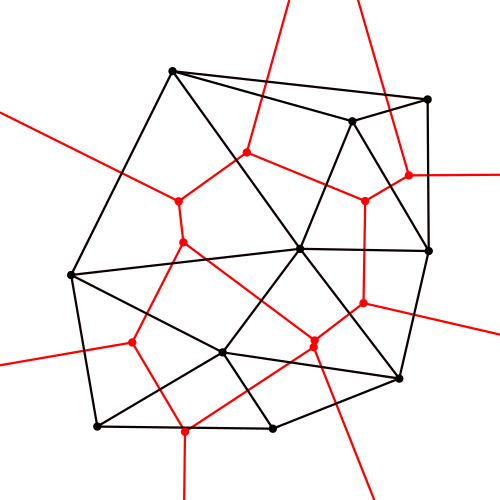
\includegraphics[width=3.45cm]{algorithms.png}
\end{wrapfigure}
\noindent
\textbf{Jury de thèse : } \\  \\
Prof.~Stefan Langerman (Université libre de Bruxelles, Président) \\
Prof.~Samuel Fiorini (Université libre de Bruxelles, Secrétaire) \\
Prof.~Jean Cardinal (Université libre de Bruxelles, Promoteur) \\
Prof.~John Iacono (Université libre de Bruxelles) \\
Prof.~Moshe Lewenstein (Bar Ilan University) \\
Prof.~Nabil Mustafa (ESIEE Paris) \\

\afterpage{\blankpage}
\end{document}
